\newcommand{\bitmap}{\proc{bmap}}
\newcommand{\pcounting}{\proc{Contagem Probabilística}}
\newcommand{\pc}{\textsf{ProbabilisticCounting}}
\newcommand{\pcpp}{\textsf{ProbabilisticCounting{++}}}

\chapter{Contagens Probabilísticas}
\label{lab:flajolet-martin}

Na seção anterior, abordamos a solução de Morris para o problema da contagem aproximada, que tinha como objetivo 
principal, estimar a quantidade de dados que passaram por um fluxo. Os fatos de, no contexto vivenciado por Morris, não 
ser possível armazenar todos os elementos nem manter a contagem em uma variável por conta de não existirem máquinas com 
registradores maiores que 8 bits tornam esse problema interessante.

Contudo, no contexo atual, em que os programas têm a disposição inteiros de 32 bits ou 64 bits, o problema da contagem
aproximada parece não ser relevante. A razão disso é que o custo para mantermos um simples contador é praticamente nulo 
nos dias atuais, de modo que, uma solução probabilística não seria tão benéfica do ponto de vista do consumo de memória.
Mesmo que esse problema não tenha aplicações imediatas atualmente, a solução proposta por Morris contém aspectos que 
inspiraram soluções de problemas mais desafiadores. Um desses problemas é descobrir o número aproximado de elementos 
distintos em um fluxo de dados~$\Mbb$. 

\begin{quote}
  \textbf{Problema} da \proc{ContagemDistintaAproximada($\Mbb$, $k$):} Dado um fluxo de dados com repetições
  $\Mbb = \{ x_1, x_2, \dots, x_s, \dots \}$, \textbf{encontrar} estimador $\hat{n}$ para o número~$n$ de elementos 
  \textit{distintos} de $\Mbb$ usando não mais que $k$ bits.
\end{quote}

Um modo de encontrarmos \textit{exatamente} a quantidade de elementos distintos de~$\Mbb$ é inserir cada item novo que 
for aparecendo em um tabela e assim, o tamanho desta tabela será a resposta para o problema. A fragilidade dessa solução 
é o consumo de memória proporcional ao número de elementos distintos, e isto pode ser uma grande limitação em situações 
nas quais existam vários fluxos sendo monitorados. 

Em muitos casos, não precisamos do valor \textit{exato} da quantidade de elementos distintos em $\Mbb$. Podemos assim, 
tentar projetar algoritmos \textit{aproximados} e que consomem muito menos memória. Uma das primeiras soluções para o 
problema da contagem distinta aproximada foi elaborada por Philippe Flajolet e Nigel Martin~\citep{flajolet:martin:85}. 
A motivação inicial desses autores era otimizar pesquisas em banco de dados relacionais, e a principal dificuldade nesse 
processo era calcular o número de elementos distintos em uma coluna. Nas próximas seções, veremos o algoritmo 
desenvolvido por Flajolet e Martin, conhecido como \proc{Contagem Probabilística}.

\section{Algoritmo da \proc{Contagem Probabilística}}
\label{sec:flajolet-martin:algorithm}

O algoritmo da \proc{Contagem Probabilística} supõe a existência uma função de hash~$h$ que associa uniformemente cada 
elemento do fluxo $\Mbb$ para um número inteiro entre $0$ e $2^L-1$ inclusive, em que $L$ é a quantidade de bits que 
cada hash possui. O algoritmo também utiliza a função $\rho$ que recebe um inteiro $y$ de $L$ bits e devolve a posição 
indexada do zero do dígito~1 menos significativo da representação binária de $y$. Vamos ver exemplos dessa função para 
$L = 4$. Temos que $\rho(12) = \rho(0011_2) = 2$ e $\rho(9) = \rho(1001_2) = 0$. Um caso particular é quando $y = 0$, e 
nesta situação, $\rho(0) = L$. E teremos um vetor $\bitmap$ de tamanho $L + 1$ inicializado com zeros.

Assim, para cada $x_i$ em $\Mbb$, cacularemos um inteiro $y_i \coloneqq h(x_i)$. Em seguida, encontraremos o valor de 
$\rho(y_i)$ e setaremos a posição $\rho(y_i)$ do vetor $\bitmap$ para $1$. Dessa forma, esse vetor guardará quais valores 
$\rho(h(x_i))$ aparecem no fluxo $\Mbb$.

Por fim, seja $R$ o menor índice tal que $\bitmap[R] = 0$. A estimativa para o número de elementos distintos de 
$\Mbb$ será $2^R/\phi$, em que, $\phi$ é um fator de correção cujo valor é $0.77351{\dots}$ e cuja origem pode ser vista
detalhadamente em ~~\citep{flajolet:martin:85}.

Vamos ver um exemplo de execução do algoritmo descrito acima. Considere que $\Mbb = \{ 4, 6, 8, 6, 9, 14 \}$, $L = 4$ e
que a função $h$ é a identidade, ou seja, para todo $x_i$, temos que $h(x_i) = x_i$. Na primeira iteração, $x_1 = 4$ e 
$\rho(4) = \rho(0010_2) = 2$. Assim, setamos $\bitmap[2] = 1$. Agora, na segunda iteração, 
$\rho(x_2) = \rho(6) = \rho(0110_2) = 1$, e setamos $\bitmap[1] = 1$. Na terceira iteração, temos que 
$\rho(x_3) = \rho(8) = \rho(0001_2) = 3$ e portanto, $\bitmap[3] = 1$. Na quarta iteração, o elemento $6$ já apareceu, 
então $\bitmap$ permanece intacto. Na iteração seguinte, $\rho(x_6) = \rho(9) = \rho(1001_2) = 0$ e $\bitmap[0] = 1$.
Na última iteração, $\rho(x_7) = \rho(14) = \rho(0111_2) = 1$, mas a posição 1 de $\bitmap$ já esta setada e dessa forma,
$\bitmap$ permance o mesmo. Falta, por fim, encontrar o valor de $R$. Como as posições 0, 1, 2, e 3 de $\bitmap$ estão
preenchidas, temos que $R = 4$ e que a estimativa do número de elementos distintos de $\Mbb$ é 
$2^{R}/\phi = 2^4/0.77351 \approx 21$. A estimativa anterior está muito distante do valor real, que é $5$. Nas seções
seguintes verificaremos se essa situação se repete para fluxos com muito mais elementos.

O algoritmo $\pc$ a seguir recebe um fluxo $\Mbb = \{ x_1, x_2, \dots, x_s, \dots \}$ com $n$ elementos distintos, 
um inteiro $L$ que representa quantos bits cada hash possui e uma função de hash~$h$ que mapeia os elementos $\Mbb$ 
para inteiros entre $0$ e $2^L - 1$ inclusive. E esse algoritmo devolve estimador $\hat{n}$ para $n$ da forma 
$2^{R}/\phi$, em que, $R$ é um número inteiro e $\phi$, uma constante teórica. Veremos mais adiante que 
$\Ebb(R) = \lg \phi n$, $\phi = 0.77351{\dots}$ e $\sigma(R) = 1.12$.

\begin{codebox}
  \Procname{$\pc(\Mbb, h, L)$}
  \li \For i de $0$ até $L + 1$
      \Do
  \li    $\bitmap[i] \gets 0$
      \End
  \li \For cada $x$ em $\Mbb$                               \label{li:pc:for:start}
      \Do
  \li   $y \gets h(x)$
  \li   $\bitmap[\rho(y)] \gets 1$                          \label{li:pc:for:end}
      \End
  \li $R \gets \{ \min 0 \leq i \leq L: \bitmap[i] = 0 \}$  \label{li:pc:r:def}
  \li\Return $2^R \mathbin{/} \phi$
  \End
\end{codebox}

O consumo de espaço do algoritmo~$\pc$ depende principalmente do vetor $\bitmap$. Os valores que podemos encontrar neste
vetor são zero, quando um dado valor de $\rho$ ainda não tiver aparecido, ou um, caso contrário. Nesse sentido, é 
possível gastarmos somente um bit para guardar essa informação. Esse algoritmo, portanto, tem um consumo de memória de 
pelo menos $O(L)$~bits.

\section{Padrões nos bits}
\label{sec:flajolet-martin:pattern}

Na seção anterior, descrevemos o algoritmo da \proc{Contagem Probabilística}. Vamos, agora, tentar entender a intuição
por trás dessa solução.

No algoritmo $\pc(\Mbb, h, L)$, a função~$h$ que mapeia uniformemente os elementos do fluxo $\Mbb$ para inteiros entre 
$0$ e $2^L - 1$ inclusive nos permite supor que o fluxo $\Mbb$ é na verdade um fluxo de números inteiros no intervalo 
$[0, 2^L - 1]$. Nesse sentido, podemos considerar um fluxo $\Mbb_h = \{ h(x_1), h(x_2), \dots, h(x_s), \dots \} = 
\{ y_1, y_2, \dots, y_s, \dots \} $, em que $x_1, x_2, \dots$ são elementos de $\Mbb$.

Dessa forma, um elemento $y_i$ de $\Mbb_h$ pode ser visto como uma palavra binária aleatória de $L$ bits em que cada bit 
é gerado independentemente com probabilidade $1/2$. Com esta interpretação, a função $\rho$ agrupa essas palavras de $L$ 
bits de acordo com seus prefixos. Assim, as palavras $z_0$ tais que $\rho(z_0) = 0$ são aquelas cujo primeiro dígito 
é~1, ou seja, tem prefixo da forma $0^01$. Já as palavras $z_1$ tais que $\rho(z_1) = 1$ são aquelas cujo bit ligado 
menos significativo está na segunda posição, ou em outros termos, tem prefixo da forma $0^11$. As palavras aleatórias de 
$L$ bits podem, portanto, ser divididas em grupos de acordo com prefixos da forma $0^{*}1$.

Se os bits de uma palavra aleatória são gerados independentemente e uniformemente, então para $R \geq 0$, a 
probabilidade de uma palavra ter um prefixo da forma $0^{R}1$ é $1/2^{R + 1}$. Probabilidade e Contagem são áreas da 
Matemática muito relacionadas, de modo que ao invés de nos perguntarmos qual a probabilidade de uma palavra ter um 
prefixo da forma $0^{R}1$, podemos nos questionar quantas palavras tem esse prefixo. Neste caso, $1/2^{R+1}$ das 
palavras terão esse prefixo.

Assim, para um fluxo $\Mbb_h$ com $n$ elementos distintos, é possível se perguntar quantos destes elementos começam com
o dígito 1. A resposta para esta pergunta é que \textbf{esperamos} que $n \mathbin{/} 2$ palavras desse fluxo se iniciem 
com o dígito 1. E $n \mathbin{/} 2^2 = n \mathbin{/} 4$ palavras devem ter o prefixo $0^{2-1}1 = 01$. Da mesma maneira, 
$n \mathbin{/} 2^3 = n \mathbin{/} 8$ palavras devem possuir um prefixo da forma $0^{3-1}1 = 001$. O vetor $\bitmap$, 
desse modo, armazena quais prefixos já apareceram no fluxo $\Mbb_h$. Falta, agora, entender o papel da variável $R$.

Suponha que $R = 4$, ou seja, $\bitmap[R] = 0$ e para $0 \leq i < R$, $\bitmap[i] = 1$. Vamos usar a ideia vista acima
para tentar estimar o número de elementos distintos que devem ter aparecido. Esperamos que $1 \mathbin{/} 2$ dos 
elementos de $\Mbb_h$ se iniciem com o dígito 1, logo, a cada dois elementos sorteados ao acaso de $\Mbb_h$, pelo menos 
um deve começar com 1. Em outras palavras, devem ter aparecido pelos menos duas palavras para que $\bitmap[0] = 1$. 
Vamos ver se esse raciocínio faz sentido para $\bitmap[1] = 1$. O esperado é que $1 \mathbin{/} 4$ dos elementos de 
$\Mbb_h$ comecem com $01$, que a cada quatro palavras sorteadas de $\Mbb_h$, pelo menos uma comece com $01$ e assim, 
devem ter aparecido quatro palavras para que $\bitmap[1] = 1$. Analogamente, devem ter aparecido pelo menos 8 palavras 
para que $\bitmap[2] = 1$ e 16 palavras para que $\bitmap[3] = 1$. Como $\bitmap[R = 4] = 0$, então ainda não devem ter 
aparecido $32$ palavras no fluxo $\Mbb_h$. Portanto, a melhor estimativa nesse caso é afirmar que $\Mbb_h$ possui 
$2^R = 16$ elementos distintos. 

A ideia descrita nessa seção é a base para os algoritmos que resolvem o problema da contagem distinta aproximada, e 
entendê-la ajudará a vermos a origem das soluções. Na próxima seção, serão expostas alguns aspectos da prova do 
funcionamento do algoritmo da $\pcounting$. 

\section{Qualidade da aproximação}
\label{sec:flajolet-martin:analysis}

Essa seção destacará as principais \textbf{etapas} da análise da~$\pcounting$ feita por Flajolet e Martin
~\citep{flajolet:martin:85}. Dessa forma, os detalhes técnicos de algums passos da demonstração podem ser explorados com 
mais detalhes a partir da leitura do artigo original. Suponha que a quantidade de elementos distintos de um fluxo $\Mbb$ 
seja~$n$. O valor esperado da variável $R$ definida na linha~\ref{li:pc:r:def} do algoritmo $\pc$ é aproximadamente 
$\lg \phi n$, em que $\phi = 0.77351{\dots}$ E o desvio padrão de $R$ é em torno de~$1.12$. 

O primeiro passo da análise é definir a variável aleatória $R_n$ como sendo o valor da variável $R$ ao final da execução 
do algoritmo~$\pc$ para uma entrada $\Mbb$ com $n$ elementos distintos, função de hash~$h$ e inteiro $L$. Assim, o 
interesse principal da demonstração é encontrar fórmulas ou estimativas para:
\begin{itemize}
  \item $p_{n,k} = \mathbb{P}(R_n = k)$: probabilidade de uma saída de $\pc$ ser igual a $k$
  \item $q_{n,k} = \mathbb{P}(R_n \geq k)$: probabilidade de uma saída de $\pc$ ser maior ou igual a $k$
  \item $\Ebb(R_n)$: valor esperado de $R_n$
  \item $\Vbb(R_n)$: variância de $R_n$
\end{itemize}

O primeiro teorema de ~\citep{flajolet:martin:85} mostra uma fórmula \textit{exata} e \textit{discreta} para $q_{n,k}$. 
A principal idea para encontrar essa fórmula é agrupar as palavras binárias por prefixos da forma $0^k1$. Nesse sentido, 
defini-se $E_k = \{ x  \ | \ \rho(x) = k \}$, ou seja, $E_k$ é o conjunto de todas as palavras aleatórias com prefixos
iguais a $0^k1$. Da mesma forma, defini-se $K_k = \{ x \ | \ \rho(x) \geq k \}$. Em seguida, as diferentes entradas 
$\Mbb$ com $n$ elementos distintos são representadas por um polinômio:
\[ P_k^{(n)} = (E_0 + E_1 + \twodots + E_{k-1} + K_k)^n .\]

O próximo passo é tentar expandir esse polinômio usando \textit{inclusão e exclusão}, e associar uma medida 
probabilidade para $E_0, E_1, \twodots, E_{k-1}, K_k$. E a prova deste teorema termina encontrando uma relação entre 
$q_{n,k}$ e esta expansão de polinômio.

Em seguida, o Teorema 2 de~\citep{flajolet:martin:85} apresenta aproximações de $q_{n,k}$ para diferentes intervalos de 
$k$. E a consequência deste teorema é  que conforme $n$ cresce, $q_{n,k}$ pode ser expresso por uma fórmula 
\textit{aproximada} e \textit{contínua}:
\[ q_{n,k} \approx \psi(\frac{n}{2^k}) \]

em que, $\psi(x) = \prod_{j \geq 0} (1 - e^{-x2^j})$.

Note que por definição, $p_{n,k} = q_{n,k} - q_{n,k+1}$. Assim, pode-se aproximar $p_{n,k}$:
\[ p_{n,k} \approx \psi(\frac{n}{2^k}) - \psi(\frac{n}{2^{k+1}}) \ . \]

O interesse passa a ser, portanto, estimar $\Ebb(R_n)$ a partir dessa fórmula aproximada de $p_{n,k}$, de maneira 
que 
\[ \Ebb(R_n) = \sum_{k \geq 1} k p_{n,k} \approx \sum_{k \geq 1} k \Big[ \psi \Big( \frac{n}{2^k} \Big) - \psi 
  \Big( \frac{n}{2^{k+1}} \Big) \Big] \ . \]

Desse modo, defini-se a função real $F(x)$ como sendo
\[ F(x) =  \sum_{k \geq 1} k \Big[ \psi \Big( \frac{n}{2^k} \Big) - \psi \Big( \frac{n}{2^{k+1}} \Big) \Big] \ . \]

E o Lema 1 do artigo, afirma que 
\[ \Ebb(R_n) = F(x) + O \Big( \frac{1}{n^{0.49}} \Big) \ , \]
ou seja, que o valor esperado de $R_n$ se aproxima de $F(x)$ conforme $n$ cresce.

Em seguida, o Lema 2 apresenta o resultado da \hyperref[ap:mellin]{transformada de Mellin} de $F(X)$. A principal razão 
para se calcular essa transformação é que podemos expressar a fórmula inversa da transformada de Mellin, que é 
$\Ebb(R_n)$, como uma expansão assintótica cujos termos são resíduos dessa transformada. Assim, o Teorema $3A$ utiliza 
os Lemas 1 e 2, e o Teorema dos Resíduos para afirmar que 
\[ \Ebb(R_n) = \lg \phi n + P(\lg n) + o(1) \ , \]
em que, $P(x)$ é a expansão assintótica de $F(x)$ e $\phi = 0.77351{\dots}$, concluindo a prova que 
$\Ebb(R_n) \approx \lg \phi n$.

A prova para a estimativa de $\Vbb(R_n)$ segue os mesmos passos da prova anterior. Pela definição de 
\hyperref[ap:variance]{variância}, precisamos estimar $\Ebb(R_n ^ 2)$. Assim, 
\[ \Ebb(R_n ^ 2) = \sum_{k=1} k^2 p_{n,k} \approx G(x) \ , \]
em que
\[ G(x) = \sum_{k=1} k^2 p_{n,k} \ . \]

Dessa forma, encontramos a transformada de Mellin de $G(x)$ e analisamos a inversa desta transformação para estimar 
$\Ebb(R_n^2)$.

\section{\proc{Lei dos Grandes Números} novamente}

Na seção anterior, foi visto que $\Ebb(R_n) \approx \lg \phi n$, em que $\phi \approx 0.77351$. Assim, se o valor 
do contador $R$ no final do algoritmo~$\pc$ para uma entrada com $n$ elementos distintos for aproximadamente igual a 
$\lg \phi n$, então a saída desse algoritmo é aproximadamente $n$. A Tabela \ref{tab:flajolet} mostra que, em alguns 
casos, a saída do programa é praticamente igual a $n$ quando $R_n \approx \lg \phi n$.

\begin{center}
  \def\arraystretch{2}%
  \begin{table}
    \begin{tabular}{ |p{1.5cm}||p{2.5cm}|  }
      \hline
      \multicolumn{1}{|p{1.5cm}|}{\centering $n$ } 
      & \multicolumn{1}{|p{2.5cm}|}{\centering $2^{\lg(\phi n)} \slash \phi$}  \\
      \hline
      \multicolumn{1}{|p{1.5cm}|}{\centering 50 } 
      & \multicolumn{1}{|p{2.5cm}|}{\centering 49.99 }  \\
      \hline
      \multicolumn{1}{|p{1.5cm}|}{\centering 500 } 
      & \multicolumn{1}{|p{2.5cm}|}{\centering 500.0 }  \\
      \hline
      \multicolumn{1}{|p{1.5cm}|}{\centering 5000 } 
      & \multicolumn{1}{|p{2.5cm}|}{\centering 4999.99 }  \\
      \hline
      \multicolumn{1}{|p{1.5cm}|}{\centering 50000 } 
      & \multicolumn{1}{|p{2.5cm}|}{\centering 50000.0 }  \\
      \hline
     \end{tabular}
     \caption{\label{tab:flajolet} Comparação entre $n$ e a saída do algoritmo~$\pc$ quando $R_n \approx \lg \phi n$.}
  \end{table}
\end{center}

Contudo, $\sigma(R_n) \approx\nolinebreak 1.12$, ou seja, o valor de $R_n$ pode ser uma unidade maior ou menor que 
$\lg \phi n$, o que implica que a estimativa de $n$ possa ser duas vezes maior ou menor que $n$. Logo, o algoritmo $\pc$ 
apresenta uma grande variabilidade.

De modo similar ao que foi visto em \hyperref[sec:morris:plus]{\proc{Morris} e a \proc{Lei dos Grandes Números}}, 
podemos obter a partir do algoritmo~$\pc$, uma solução com variância menor. Assim, o algoritmo $\pc{+}$ recebe um fluxo 
de dados $\Mbb$, inteiros $m$ e $L$, além de uma lista de $m$ funções de hash $\mathbb{H}$, em que cada função 
$\mathbb{H}_i$ desse grupo mapeia uniformemente os elementos de $\Mbb$ para o intervalo $[0, 2^L - 1]$. Esse algoritmo 
modificado manterá $m$ vetores $\bitmap$, de maneira que para cada elemento $x$ de $\Mbb$, para todo $0 \leq j < m$, 
vamos setar $\bitmap_j[\rho(\mathbb{H}_{j}(x))] = 1$. Quando todos os itens de $\Mbb$ forem percorridos, calcularemos 
$R_j = \{ \min 0 \leq i \leq L: \bitmap_{j}[i] = 0 \}$ para todo $0 \leq j < m$ e em seguida, encontraremos a média 
desses valores obtendo $\overline{R}$. Por fim, a estimativa para o número de elementos distintos em $\Mbb$ será 
$2^{\overline{R}} \mathbin{/} \phi$. 

Uma outra forma de vermos essa solução é que estamos executando em pararelo $m$ funções $\pc$ e para isso, temos que 
passar uma função de hash diferente para cada execução, a fim de produzir vetores $\bitmap$ diferentes ao final.

\begin{codebox}
  \Procname{$\pc{+}(\Mbb, \mathbb{H}, L, m)$}
  \li \For $j$ de $0$ até $m$
      \Do
  \li    \For $i$ de $0$ até $L + 1$
          \Do
  \li       $\bitmap_{j}[i] \gets 0$
          \End
      \End
  \li \For $j$ de $0$ até $m$
      \Do
  \li    \For cada $x$ em $\Mbb$
          \Do
  \li       $y \gets \mathbb{H}_{j}(x)$
  \li       $\bitmap_j[\rho(y)] = 1$
          \End
      \End
  \li \For $i$ de $0$ até $m$
      \Do
  \li    $\mathbb{R}[j] = \{ \min 0 \leq i \leq L: \bitmap_{j}[i] = 0 \}$
      \End
  \li $\overline{R} = \sum_{j=0}^{m-1} \mathbb{R}[j] \mathbin{/} m$
  \li \Return $2^{\overline{R}} \mathbin{/} \phi$
  \End
\end{codebox}

Seja $\overline{R_n}$ o valor da variável $\overline{R}$ ao final da execução do algoritmo~$\pc{+}$ para uma
entrada com $n$ elementos distintos. De forma análoga aos resultados vistos em \hyperref[sec:morris:plus]{\proc{Morris} 
e a \proc{Lei dos Grandes Números}}, podemos concluir que:
\[ \Ebb(\overline{R_n}) \approx \lg \phi n   \; \; \text{e}  \; \; \sigma(\overline{R_n}) \approx \frac{1.12}{\sqrt{m}} \ . \]

No entanto, o fato de precisarmos de uma função de hash distinta para cada iteração torna a solução acima inviável, uma 
vez que, encontrar funções que mapeiem na prática os elementos de um fluxo $\Mbb$ de maneira uniforme não é uma 
tarefa simples. Para contornar esse problema, os autores propuseram o uso da \textbf{média estocástica}.

Essa ideia consiste em dividr os elementos da entrada em $m$ lotes e usar parte da informação do hash dos elementos para 
definir em qual lote um elemento deve ir. As linhas \ref{li:pcpp:for:start}-\ref{li:pcpp:for:end} do algoritmo~$\pcpp$ 
a seguir mostram como essa divisão é feita.

\begin{codebox}
  \Procname{$\pcpp(\Mbb, $h$, $L$)$}
  \li \For $j$ de $0$ até $m$
      \Do
  \li    \For $i$ de $0$ até $L + 1$
          \Do
  \li       $\bitmap_{j}[i] \gets 0$
          \End
      \End
  \li \For cada $x$ em $\Mbb$                                                         \label{li:pcpp:for:start}
      \Do
  \li   $\texttt{lote} \gets h(x) \bmod k$
  \li   $y \gets \lfloor h(x) \mathbin{/} k \rfloor$
  \li   $\bitmap_{\texttt{lote}}[y] = 1$                                              \label{li:pcpp:for:end}
      \End
  \li \For $i$ de $0$ até $m$
      \Do
  \li    $\mathbb{R}[j] = \{ \min 0 \leq i \leq L: \bitmap_{j}[i] = 0 \}$             \label{li:pcpp:rmin}
      \End
  \li $\overline{R} = \sum_{j=0}^{m-1} \mathbb{R}[j] \mathbin{/} m$
  \li \Return $m \ \times \ 2^{\overline{R}} \mathbin{/} \phi$
  \End
\end{codebox}

Se a função de hash $h$ distribuir os $n$ elementos distintos do fluxo $\Mbb$ uniformemente entre os $m$ lotes, então 
esperamos que cada lote tenha aproximadament $\frac{n}{m}$ elementos. Nesse caso, $2^{\overline{R_n}} \mathbin{/} \phi$ 
seria uma aproximação para $\frac{n}{m}$. É devido a este fato que a saída do algoritmo~$\pcpp$ é 
$\mathbf{m} \ \times \ 2^{\overline{R_n}} \mathbin{/} \phi$, pois este valor é uma estimativa para 
$\mathbf{m} \ \times \ \frac{n}{m} = n$. 

Na Seção~\ref{sec:flajolet-martin:algorithm}, vimos que no algoritmo~$\pc$, precisamos de pelo menos $O(L)$ bits para 
armazenarmos o vetor $\bitmap$. Como o algoritmo~$\pcpp$ tem $m$ vetores $\bitmap$, o custo de espaço dele é de pelo 
menos $O(mL)$ bits.

Por fim, o desvio padrão do algoritmo $\pcpp$ é em torno de $0{,}78 \mathbin{/} \sqrt{m}$. Isto quer dizer que para 
$m = 64$, o desvio esperado é em torno de $10\%$. Dessa forma, a escolha de $m$ depende das exigências do problema. Se 
precisarmos de uma precisão maior, escolheremos um valor de $m$  maior, mas teremos um algoritmo mais custoso em termos 
de tempo e espaço. Por outro lado, se a exigência é, por exemplo, decidir qual de dois conjuntos tem a menor quantidade 
de elementos distintos, podemos escolher um valor menor de $m$ para fazer essa comparação, mesmo tendo um risco maior de 
escolher o conjunto errado.

\section{Estimando valores pequenos com a \proc{Contagem Probabilística}}
\label{sec:fm:low_estimates}

Uma das principais razões para escolhermos algoritmos \textit{probabilísticos} ao invés de algoritmos \textit{exatos} é 
o \textbf{consumo de memória reduzido}. Como já foi abordado, para resolver o problema da contagem distinta de forma 
\textit{exata}, podemos manter uma tabela de hash e conforme os elementos forem processados, adicionar a esta tabela 
somente aqueles elementos que não apareceram ainda. Assim, a quantidade de elementos distintos processados será o tamanho 
da tabela. Suponha que cada hash seja um inteiro de 4 bytes (32 bits) e que existam um milhão de itens distintos 
percorridos. Para armazenar essa tabela, gastaríamos pelos menos 4 MB. Por outro lado, se usarmos o algoritmo da
$\pcounting$ para resolver esse problema, o consumo de memória seria proporcional ao valor $m$ e não dependeria da 
quantidade de itens distintos. Suponha que $\bitmap$ seja um vetor de bits e que tenhamos $m$ vetores deste tipo. Se $m$ 
for igual a 1024, então a memória consumida por esse algoritmo seria em torno de 4 KB, que é um consumo de espaço
\textbf{1000 vezes menor} que a solução exata.

O desvio padrão da $\pcounting$ para $m = 1024$ é em torno de $2{,}5\%$. Logo, para um fluxo de milhões de itens 
distintos, o erro esperado seria em torno das dezenas ou centenas de milhares. Com esse tipo de desvio, teríamos como 
mensurar a ordem de grandeza do número de itens distintos que já passaram por um fluxo com bastante confiança. Contudo, 
para utilizar a $\pcounting$, o viés desse algoritmo deve ser entendido.

O \textbf{viés} de um estimador é a diferença entre seu valor esperado e o valor real do parâmetro estimado. 
Nesse sentido, a estimativa da quantidade de elementos em um conjunto devolvida pelo algoritmo de \proc{Morris} é 
\textit{não-viesada}, uma vez que, o \hyperref[morris:theorem:expected_value]{Teorema do valor esperado de $\Morris$} 
afirma que o valor esperado deste estimador é igual ao tamanho do conjunto estimado.

Na prova descrita em ~\citep{flajolet:martin:85}, o estimador de $\lg n$ é $R_n$, que representa o valor da variável 
$R$ ao final da execução de \proc{ProbabilisticCounting}, tendo como entrada um fluxo de dados com $n$ elementos 
distintos. Vimos que o valor esperado de $R_n$ é aproximadamente $\lg \phi n$, que é diferente de $\lg n$. Portanto, 
$R_n$ é um estimador \textit{viesado} de $\lg n$. E analogamente, o estimador devolvido por $\pcpp$ também é 
\textit{viesado}.  

Então, além do erro padrão, existe também o viés do algoritmo da \proc{Contagem Probabilística}, cujo valor é 
$1 + 0{,}31 \mathbin{/} m$. Contudo, para valores de $m$ maiores que $32$, o viés se torna desprezíval se comparado ao 
desvio padrão. Dessa forma, uma pessoa pode ser induzida a concluir que a escolha de $m$ é o único cuidado que ela deve 
tomar ao utilizar esse algoritmo. No entanto, ainda existe o problema de estimar \textbf{baixas cardinalidades} com essa 
estrutura.

Suponha, portanto, que $m = 64$ e que o hash do único elemento que já passou por um fluxo $\Mbb$ comece com $1$. Logo, 
se passarmos $\Mbb$ para $\pcpp$, existiria um vetor $\bitmap$ cuja primeira posição teria o valor $1$, e o restante dos 
vetores $\bitmap$ teriam todos valores zero. Assim, $\overline{R}$ seria igual a $1 \mathbin{/} 64$, e o estimador de 
$n$ teria o valor de $64 \ \times \ 2^{\frac{1}{64}} \mathbin{/} \phi \approx 83.64$. Esta estimativa está 
muito distante do valor real, que é $n = 1$.

Em vista disso, um tratamento especial deve ser dado para situações em que a cardinalidade do número de elementos 
distintos de um conjunto for baixa. Poderíamos, por exemplo, manter os elementos percorridos em uma tabela de hash, e 
quando essa tabela atingisse um certo tamanho, passaríamos a usar a estratégia original da $\pcounting$, que é preencher
os vetores $\bitmap$.  

O artigo ~\citep{flajolet:martin:85} nomeia esse problema como \textbf{não-lineariade inicial}, e os autores afirmam que 
a estimativa se aproxima do valor esperado do estimador assim que a quantidade de elementos distintos atinge pelo menos 
os valores $10m{-}20m$. Assim, para $m = 64$, é esperado que essa imprecisão inicial desapareça quando aproximadamente 
$600{-}1200$ dados distintos passarem pelo fluxo.

Vale lembrar, no entanto, que a proposta inicial para a adoção de estruturas de dados probabilísticas é o alto consumo 
de memória conforme o volume dos dados cresce. Nesse sentido, esse problema da não-linearidade inicial pode ser 
desconsiderado dependendo da situação. 

\section{Implementando $\pcounting$}
\label{sec:fm:experiments}

Nesta seção, apresentaremos a implementação da $\pcounting$. Além disso, experimentos similares ao da 
Seção~\ref{chap:morris:experiments} forams realizados com o objetivo de se verificar a acurácia dessa solução.

A implementação foi baseada no algoritmo $\pcpp$ com algumas modificações. Dessa forma, definimos uma 
classe~\texttt{ProbabilisticCounting}, cujo construtor recebe os parâmetros $m$ e $L$. E nesta classe, existem os 
métodos \texttt{adiciona} e \texttt{conta}. O primeiro adiciona um elemento à estrutura, e o segundo devolve a 
estimativa da quantidade de elementos distintos. Assim, as simulações se baseiam em uma versão \textit{online} da 
$\pcounting$ para que possamos observar como a estimativa evolui conforme novos itens são inseridos nessa estrutura.

\newpage
\begin{lstlisting}[style=mypython,caption=Implementação do algoritmo $\pcpp$,captionpos=b, label=pc:code]
class ProbabilisticCounting:
    def __init__(self, m=64, L=64):
        self.m: int = m
        self.L: int = L
        self.phi = 0.77351
        self.BITMAP: List[List[int]] = []

        for _ in range(0, self.m):
            self.BITMAP.append([None] * self.L)

        self.R: List[int] = [0] * self.m
        self.R_sum = 0

    def p(self, x: int):
        return (x & -x).bit_length() - 1

    def adiciona(self, x: int):
        lote = x % self.m
        y = x // self.m
        self.BITMAP[lote][self.p(y)] = 1

        while self.BITMAP[lote][self.R[lote]] == 1:
            self.R[lote] += 1
            self.R_sum += 1

    def conta(self):
        R = self.R_sum / self.m

        return floor((self.m * pow(2, R)) / self.phi)
\end{lstlisting}

Vamos comentar alguns detalhes de implementação do Programa~\ref{pc:code}. O primeiro deles é relacionado ao método
~\texttt{adiciona}, que foi baseados nas linhas~\ref{li:pcpp:for:start}--\ref{li:pcpp:rmin} do algoritmo~$\pcpp$. O 
principal diferencial da implementação desse método na classe~\texttt{ProbabilisticCounting} é que já mantemos o menor
valor de $R$ de cada lote atualizado, como pode ser visto no \texttt{while}. Dessa forma, a complexidade de se adicionar
um elemento nessa estrutura é $O(1)$ amortizado.

O próximo comentário é relacionado ao método \texttt{p} da classe \texttt{ProbabilisticCounting}, que é a implementação 
da função $\rho$ do algoritmo~$\pcpp$. Essa função deve retornar a posição do bit ligado menos significativo de um 
inteiro. Assim, dado um inteiro~$x$, tentaremos encontrar uma forma de encontrar o índice do bit ligado menos 
significativo de $x$. É interessante, portanto, considerar o oposto de $x$, ou seja, $-x$. Considerando a representação 
binária de $x$, $-x$  pode ser calculado da seguinte maneira: $\overline{x} + 1$, em que $\overline{x}$ é o complementar 
de $x$, cuja representação binária inverte todos os bits de $x$. Tendo $-x$ em mãos, a posição do único bit ligado de 
$x \ {\&} \ {-x}$ coincide com a posição do bit ligado menos significativo de~$x$. Para recuperarmos esse bit de 
$x \ {\&} \ {-x}$ , usamos a função \texttt{bit\_length} do \proc{Python} que retorna a menor quantidade de bits para se 
representar um inteiro. Esta função é indexada a partir do 1 e, por isso, subtraímos 1 do retorno dela. 

Vamos ver alguns exemplos para deixar essa ideia mais clara. Tome $\rho(10) = \rho(0101_2) = 1$. Para chegar nesse valor 
de 1, primeiro encontramos $-10 = \overline{10} + 1 = 1010_2 + 1000_2 = 0110_2$. Em seguida, calculamos
$10 \ {\&} \ {-}10 = 0101_2 \ {\&} \ 0110_2 = 0100_2$. E a posição do único bit ligado deste número binário é 1. Outro 
exemplo é $\rho(9) = \rho(1001_2) = 0$. Assim, $-9 = \overline{9} + 1 = 0110_2 + 1000_2 = 1110_2$, e 
$9 \ {\&} \ {-}9 = 1001_2 \ {\&} \ 1110_2 = 1000_2$. E o único bit ligado deste número está na posição zero, que coincide 
com o valor de $\rho(9)$.

Outro detalhe de implementação é que não estamos utilizando a função de hash~$h$ durante a inserção dos elementos na 
estrutura, uma vez que, os elementos inseridos já são inteiros, e estamos supondo que eles são gerados uniformemente. 
Assim, não há a necessidade de mapeá-los para inteiros entre $0$ e $2^{L} - 1$, inclusive. Ou seja, implicitamente, 
temos que $h$ é a função identidade.

Tendo esclarecido os detalhes de implementação do Programa~\ref{pc:code}, podemos partir para a apresentação dos 
experimentos. O valor de $L$ utilizado nesses experimentos foi de $64$, uma vez que, a maior parte das linguagens de 
programação suporta atualmente inteiros de $8$~bytes. Além disso, gerar número aleatórios de 64 bits garante uma maior
variabilidade dos dados dos experimentos. 

O primeiro experimento tem como objetivo verificar a evolução da estimativa devolvida pela estrutura 
conforme mais elementos são inseridos nela. Dessa forma, realizamos uma simulação em que geramos um milhão de inteiros 
aleatórios que foram sendo inseridos em uma estrutura~\texttt{ProbabilisticCounting}. Essa simulação foi repetida duas 
vezes, sendo que na primeira, os elementos foram inseridos em um estrutura com $m = 64$ e na segunda vez, os mesmos 
itens foram adicionandos à estrutura com $m = 1024$. Os resultados dessas simulações estão presentes na 
Figura~\ref{fig:pc:experimento:01}. Analisando primeiramente, as estimativas da estrutura com $m = 64$, podemos notar 
que as estimativas, que são representadas pela linha laranja, ficaram levemente distantes dos valores reais, que são 
representados pela linha azul. Outro fato notável é que ao aumentarmos o valor de $m$ para $1024$, essa distância 
diminuiu, o que quer dizer que a precisão das estimativas aumentou.

\begin{figure}
  \centering
  \begin{subfigure}{.5\textwidth}
    \centering
    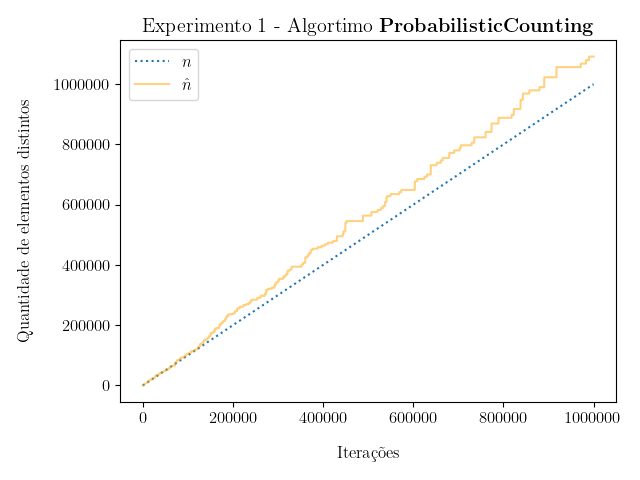
\includegraphics[width=\linewidth, height=4cm]{figuras/probabilistic_counting_full_64.png}
  \end{subfigure}%
  \begin{subfigure}{.5\textwidth}
    \centering
    \captionsetup{justification=centering}
    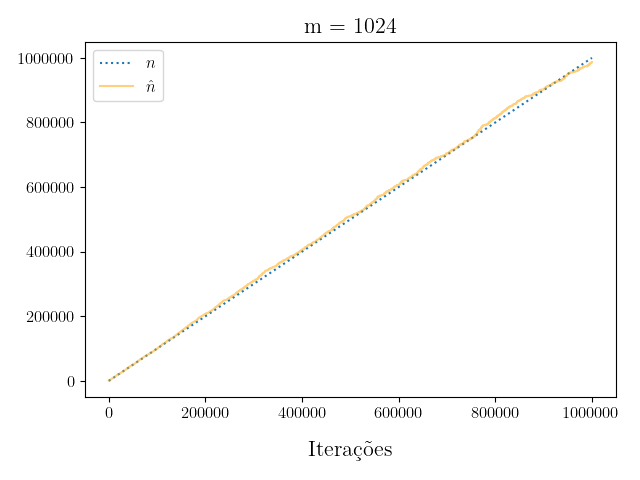
\includegraphics[width=\textwidth, height=4cm]{figuras/probabilistic_counting_full_1024.png}
  \end{subfigure}
  \caption{Primeiro experimento do algoritmo~$\pcpp$. Foram inseridos em estruturas~\texttt{ProbabilisticCounting} com 
  $m = 64$ e $m = 1024$, um milhão de inteiros de 64 bits gerados uniformemente.}
  \label{fig:pc:experimento:01}
\end{figure}


Na Seção~\ref{sec:fm:low_estimates}, vimos que a $\pcounting$ estima pequenas cardinalidades com um grande erro. Esse 
fato pode ser confirmado na Figura~\ref{fig:pc:experimento:01:first}, que destaca as estimativas iniciais das estruturas
com $m = 64$ e $m = 1024$. É possível notar que a linha das estimativas já começa distante da linha dos valoes reais e
que essa distância cresce quando o valor de $m$ aumenta.

\begin{figure}
  \centering
  \begin{subfigure}{.5\textwidth}
    \centering
    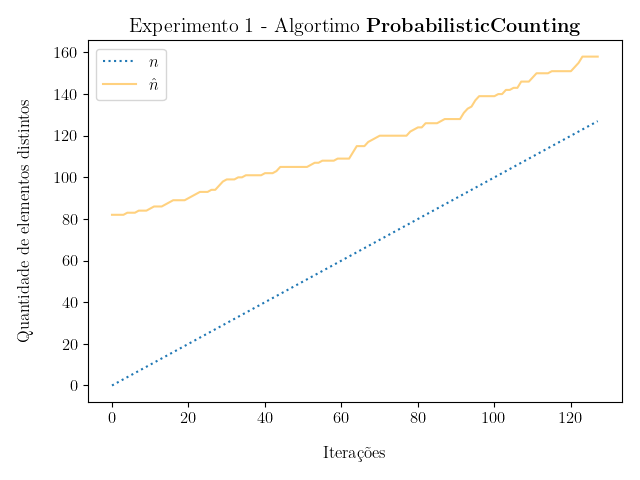
\includegraphics[width=\linewidth, height=4cm]{figuras/probabilistic_counting_first_64.png}
  \end{subfigure}%
  \begin{subfigure}{.5\textwidth}
    \centering
    \captionsetup{justification=centering}
    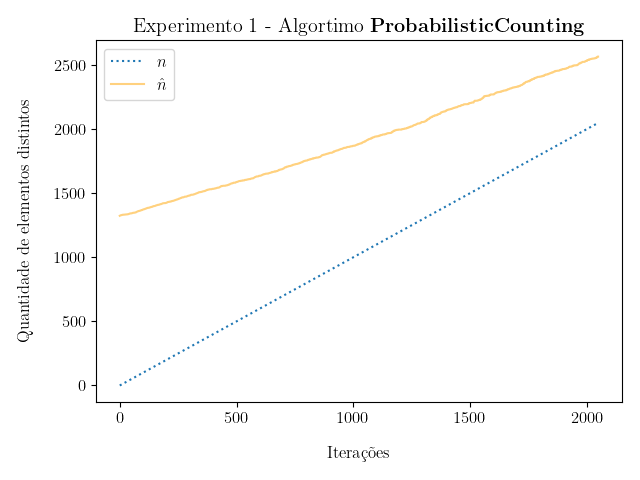
\includegraphics[width=\textwidth, height=4cm]{figuras/probabilistic_counting_first_1024.png}
  \end{subfigure}
  \caption{Primeiro experimento do algoritmo~$\pcpp$. Foram destacadas as primeiras 128 iterações da simulação com a
  estrutura~\texttt{ProbabilisticCounting} com $m = 64$ e as 2048 estimativas iniciais da simulação com a estrutura com 
  $m = 1024$. Podemos perceber que as estimativas iniciais apresentam um grande erro, que é a distância da linha laranja 
  para a linha azul.}
  \label{fig:pc:experimento:01:first}
\end{figure}

Em vista desse erro no início do algoritmo, vamos desconsiderar as primeiras iterações do experimento anterior e tentar 
observar se \texttt{ProbabilisticCounting} começa a produzir melhores estimativas conforme mais itens são inseridos 
nessa estrutura. A Figura~\ref{fig:pc:experimento:01:sem:first} exibe a evolução das estimativas devolvidas 
desconsiderando as primeiras. O desvio padrão da $\pcounting$ é de $0{,}78 \mathbin{/} \sqrt{m}$, e portanto, para 
$m = 64$, esse desvio é de $9{,}8 \%$, e para $m = 1024$, $2{,}4 \%$. Sendo assim, se desconsiderarmos as primeiras 
estimativas, a $\pcounting$ com $m = 64$ devolveu valores dentro de dois desvios padrões. Já na simulação com 
$m = 1024$, as estimativas ficaram dentro de um desvio, indicando um aumento de precisão.

\begin{figure}
  \centering
  \begin{subfigure}{.5\textwidth}
    \centering
    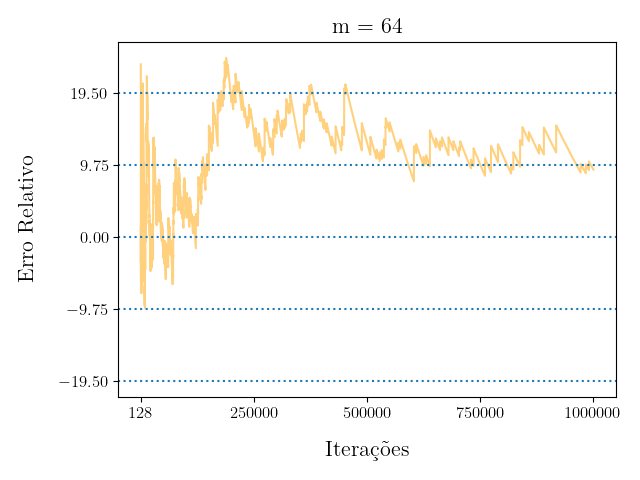
\includegraphics[width=\linewidth, height=4cm]{figuras/probabilistic_counting_erro_sem_first_64.png}
  \end{subfigure}%
  \begin{subfigure}{.5\textwidth}
    \centering
    \captionsetup{justification=centering}
    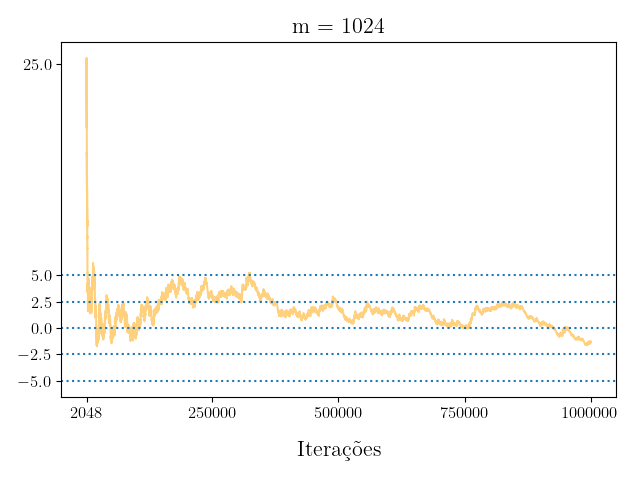
\includegraphics[width=\textwidth, height=4cm]{figuras/probabilistic_counting_erro_sem_first_1024.png}
  \end{subfigure}
  \caption{Erro relativo do primeiro experimento do algoritmo~$\pcpp$. Foram desconsideradas as primeiras 128 iterações
  da simulação com a estrutura~\texttt{ProbabilisticCounting} com $m = 64$ e as 2048 estimativas iniciais da simulação
  com a estrutura com $m = 1024$. Podemos perceber que as estimativas da estrutura com $m = 64$, ficaram 
  majoritariamente entre dois desvios padrões. Por outro lado, a maior parte dos valores devolvidos pela $\pcounting$ 
  com $m = 1024$ ficaram dentro de um desvio padrão.}
  \label{fig:pc:experimento:01:sem:first}
\end{figure}

As duas simulações apresentadas anteriormente destacam a imprecisão da estrutura~\texttt{ProbabilisticCounting} na hora 
de estimarmos pequenos valores e que aumentando o valor de $m$, essa imprecisão ficar ainda pior. Contudo, a partir de 
um certo ponto, esse problema desaparece e um parâmetro $m$ maior implica em um algoritmo mais preciso. Dessa forma, o
próximo experimento tem como objetivo verificar a variância da $\pcounting$ e como $m$ a influencia.

Assim como foi feito na Seção~\ref{chap:morris:experiments}, repetimos as simulações do primeiro experimento da 
$\pcounting$ várias vezes, e coletamos a frequência das estimativas. A Figura~\ref{fig:pc:experimento:02} exibe como as 
estimativas devolvidas pela estrutura~\texttt{ProbabilisticCounting} com $m = 64$ e $m = 1024$ ficaram distribuídas 
após dez mil simulações. Quase todas as estimativas ficaram entre dois desvios padrões nos dois casos, e os valores 
devolvidos pela estrutura com $m = 1024$ ficaram mais concentrados em torno da quantidade real de elementos distintos,
que é de um milhão. Assim, quando aumentamos o valor de $m$, estamos diminuindo a variância do algoritmo.

\begin{figure}
  \centering
  \begin{subfigure}{.5\textwidth}
    \centering
    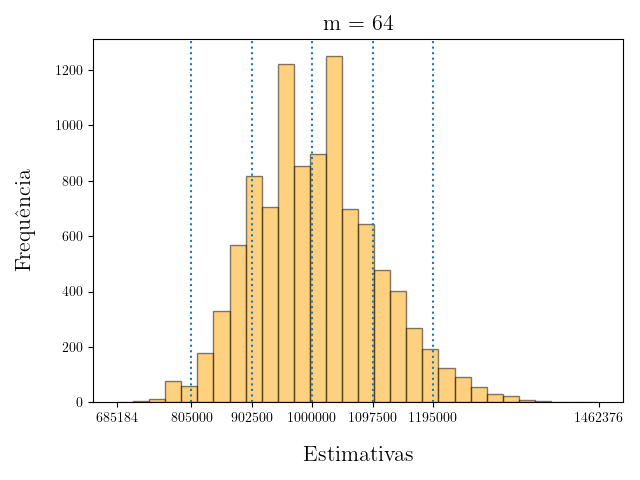
\includegraphics[width=\linewidth, height=4cm]{figuras/probabilistic_counting_variance_64.png}
  \end{subfigure}%
  \begin{subfigure}{.5\textwidth}
    \centering
    \captionsetup{justification=centering}
    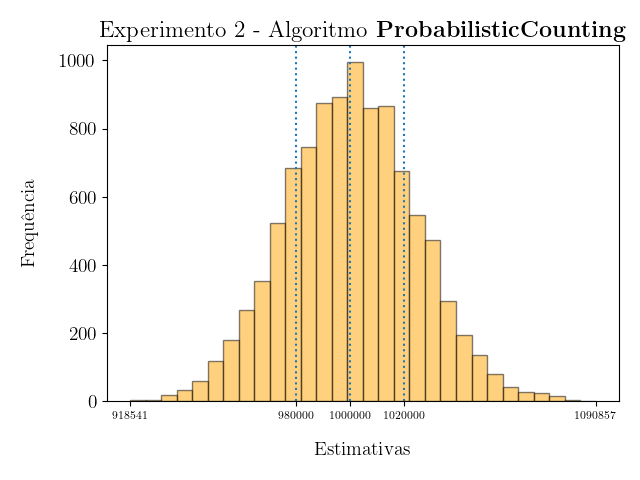
\includegraphics[width=\textwidth, height=4cm]{figuras/probabilistic_counting_variance_1024.png}
  \end{subfigure}
  \caption{Segundo experimento do algoritmo~$\pcpp$. Foram realizadas dez mil simulações, e em cada simulação, foram 
  inseridos em estruturas~\texttt{ProbabilisticCounting} com $m = 64$ e $m = 1024$, um milhão de inteiros de 64 bits 
  gerados uniformemente. Os resultados foram utilizados para a construção dos histogramas de frequência acima.}
  \label{fig:pc:experimento:02}
\end{figure}

A partir dos experimentos apresentados, foi possível termos noção da precisão do algoritmo da $\pcounting$ e como 
manipular o parâmetro~$m$ para que tenhamos resultados melhores. Conseguimos, também, observar por meio das simulações a 
\textbf{não-lineariade inicial} desse algoritmo. Contudo, mesmo com esse obstáculo, essa estrutura de dados foi de 
grande importância para que pesquisas de bancos de dados pudessem ser otimizadas, e várias ideias dela serviram de base
para que outras soluções com menor consumo de memória surgissem. E nos próximos capítulos, continuaremos vendo outros 
modos de resolvermos o problema da contagem distinta aproximada.